\documentclass[aspectratio=169,10pt]{beamer}
\usepackage[T1]{fontenc}
\usepackage[utf8]{inputenc}
\usepackage[english]{babel}
\usepackage{mathpazo,amsmath,amssymb,bm,graphicx,booktabs,array,tikz,pgfpages,microtype}
\usefonttheme{serif}
\hyphenpenalty=10000
\exhyphenpenalty=10000
\usetikzlibrary{arrows.meta,calc,positioning}
\definecolor{navy}{HTML}{183C50}
\definecolor{teal}{HTML}{147D80}
\definecolor{ochre}{HTML}{B57932}
\definecolor{muted}{HTML}{576A75}
\definecolor{pale}{HTML}{E8EFF2}
\definecolor{glide}{HTML}{315EB3}
\definecolor{search}{HTML}{BC3D48}
\definecolor{climb}{HTML}{3F855A}
\setbeamertemplate{navigation symbols}{}
\setbeamertemplate{footline}{}
\setbeamercolor{normal text}{fg=navy,bg=white}
\ifdefined\Speakernotes
  \setbeameroption{show notes on second screen=right}
\else
  \setbeameroption{hide notes}
\fi
\hypersetup{colorlinks=true,urlcolor=teal,linkcolor=teal,
 pdfauthor={Matteo Di Sante},pdftitle={Soaring flight: internship and thesis research directions}}
% Hyperlink annotations do not follow pgfpages' two-screen imposition reliably.
% The projected PDF keeps live links; the notes PDF keeps their visible text.
\ifdefined\Speakernotes\hypersetup{draft}\fi
% Generated by audit_coverage.py. Archived segmentation snapshot: 16 Sep 2026.
\newcommand{\ParaTotalFlights}{156,406}
\newcommand{\ParaClassFlights}{104,636}
\newcommand{\ParaClassFlightPct}{66.9}
\newcommand{\ParaClassFixPct}{88.2}
\newcommand{\ParaClassTimePct}{69.9}
\newcommand{\ParaLostTimePct}{30.1}
\newcommand{\ParaCadTimePct}{70.7}
\newcommand{\ParaCadFixPct}{89.3}
\newcommand{\ParaCadFlightPct}{69.9}
\newcommand{\HangTotalFlights}{6,094}
\newcommand{\HangClassFlights}{1,670}
\newcommand{\HangClassFlightPct}{27.4}
\newcommand{\HangClassFixPct}{61.7}
\newcommand{\HangClassTimePct}{29.1}
\newcommand{\HangLostTimePct}{70.9}
\newcommand{\HangCadTimePct}{29.2}
\newcommand{\HangCadFixPct}{62.0}
\newcommand{\HangCadFlightPct}{28.0}

\newcommand{\txt}[5][]{\node[anchor=north west,inner sep=0pt,text width=#4mm,align=left,font=\fontsize{10.3}{12.5}\selectfont,#1]at(#2,#3){#5};}
\newcommand{\smalltxt}[5][]{\txt[font=\fontsize{8.7}{10.7}\selectfont,#1]{#2}{#3}{#4}{#5}}
\newcommand{\head}[5][]{\txt[font=\bfseries\fontsize{11.4}{13.3}\selectfont,#1]{#2}{#3}{#4}{#5}}
\newcommand{\credit}[1]{\txt[text=muted,font=\fontsize{6.3}{7.5}\selectfont]{8}{84}{144}{#1}}
\newcommand{\ruleat}[1]{\draw[pale,line width=.6pt](8,#1)--(152,#1);}
\newcommand{\startslide}[2]{\begin{tikzpicture}[remember picture,overlay,shift={(current page.north west)},x=1mm,y=-1mm]
  \fill[white](0,0)rectangle(160,90);
  \fill[navy](0,0)rectangle(160,13);
  \node[anchor=west,text=white,inner sep=0pt,font=\bfseries\fontsize{15}{17}\selectfont]at(8,6.5){#1};
  \node[anchor=east,text=white,inner sep=0pt,font=\fontsize{8}{9}\selectfont]at(152,6.5){#2};}
\newcommand{\finishslide}{\end{tikzpicture}}
\newcommand{\arrow}[4]{\draw[-{Stealth[length=2mm]},line width=.9pt,teal](#1,#2)--(#3,#4);}
\setbeamertemplate{note page}{\vspace{3mm}\noindent
 {\color{teal}\small Internship and thesis plan\hfill Slide \insertframenumber}\par\medskip
 {\fontsize{9}{11}\selectfont\raggedright\insertnote}}

\begin{document}

% 1 — Minimal title and the actual research dependency diagram.
\begin{frame}[plain]
\begin{tikzpicture}[remember picture,overlay,shift={(current page.north west)},x=1mm,y=-1mm]
 \fill[navy](0,0)rectangle(160,90);
 \txt[text=white!72!navy,font=\fontsize{10}{12}\selectfont]{10}{12}{130}{INTERNSHIP AND MASTER'S THESIS}
 \txt[text=white,font=\bfseries\fontsize{25}{28}\selectfont]{10}{24}{140}{Soaring flight\\Research directions}
 \txt[text=white!85!navy,font=\fontsize{12}{15}\selectfont]{10}{50}{135}{Stochastic motion, collective flight\\and possible extensions to optimal control}
 \draw[white!30!navy](10,72)--(150,72);
 \txt[text=white,font=\fontsize{10}{12}\selectfont]{10}{77}{78}{Matteo Di Sante}
 \txt[text=white!80!navy,align=right,font=\fontsize{9}{11}\selectfont]{85}{77}{65}{October 2026 -- February 2027}
\end{tikzpicture}
\note{This is a proposed research programme for discussion with the supervisors. The shared foundation is segmentation and a broader stochastic description of flight. The model and solo/group comparison reuse that foundation. Optimal control is an exploratory extension whose scope depends on the data and on reading the literature. The dates are planning windows rather than promises of completed scientific conclusions.}
\end{frame}

% 2 — Shared foundation, then possible paths.
\begin{frame}[plain]
\startslide{Research paths and dependencies}{2 / 12}
 \head[text=teal]{8}{19}{144}{1\quad Data download and preprocessing: completed}
 \smalltxt{8}{27}{142}{Possible simplification of preprocessing, with checks on phase labels and measured observables.}
 \ruleat{37}
 \head{8}{43}{35}{2\quad Segmentation}
 \smalltxt{8}{52}{35}{Continuous observations\\Validated phase labels}
 \arrow{44}{49}{50}{49}
 \head{53}{42}{43}{3\quad Stochastic\\characterisation}
 \smalltxt{53}{58}{43}{A common set of empirical\\tests for all later work}
 \draw[teal,line width=.9pt](98,50)--(102,50);
 \draw[teal,line width=.9pt](102,44)--(102,64);
 \arrow{102}{44}{108}{44}
 \arrow{102}{64}{108}{64}
 \head[text=glide]{111}{39}{41}{4\quad Stochastic model}
 \smalltxt{111}{47}{41}{Intermittency and memory}
 \head[text=teal]{111}{60}{41}{5\quad Solo vs group}
 \smalltxt{111}{68}{41}{Individual and joint motion}
 \smalltxt[text=ochre]{8}{75}{144}{6\quad Exploratory extension: thermal statistics and stochastic optimal control}
 \credit{Parallel throughout: maintain and improve the graphical analysis tool.}
\finishslide
\note{Download and preprocessing already exist. Simplification should reduce unnecessary complexity while preserving the bridge-or-split rule for unsupported gaps and the quality flags used by observables. Stage 3 is fundamental: it defines which properties a candidate model must reproduce and which quantities distinguish solo and group flight. Stages 4 and 5 are scheduled consecutively but are scientifically complementary paths. The optimal-control extension also requires reliable phase labels and a defensible interpretation of observed thermal locations.}
\end{frame}

% 3 — Current constraint and concrete next work.
\begin{frame}[plain]
\startslide{Segmentation with continuous observations}{3 / 12}
 \head{8}{18}{67}{Vilpellet's current implementation}
 \smalltxt{8}{27}{67}{Three binary indicators, eight possible emissions. Windows: 6, 30 and 90 fixes. Angular thresholds and transitions are per fix.}
 \smalltxt[text=ochre]{8}{45}{67}{Calibrated near 1 Hz. The current port requires mean $\Delta t<1.2$ s. Other cadences need adaptation and validation.}
 \head[text=teal]{84}{18}{68}{12--25 October\quad [2 weeks]}
 \smalltxt{84}{27}{68}{Develop the existing Gaussian HMM prototype: continuous $v_z$, horizontal speed and turning features, measured over windows in seconds.}
 \smalltxt{84}{45}{68}{Discrete hidden phases remain. Validate labels, boundaries and durations on independent annotated flights and across cadences.}
 \ruleat{61}
 \smalltxt{8}{65}{71}{\textbf{Time currently excluded from phase analysis}}
 \txt[text=ochre,font=\bfseries\fontsize{18}{20}\selectfont]{8}{72}{67}{\ParaLostTimePct\%\ \textnormal{\fontsize{9}{11}\selectfont paragliders}}
 \txt[text=ochre,font=\bfseries\fontsize{18}{20}\selectfont]{84}{72}{68}{\HangLostTimePct\%\ \textnormal{\fontsize{9}{11}\selectfont hang gliders}}
 \credit{Archived segmentation, 16 Sep 2026. Denominator: supported cleaned time. Includes cadence and length exclusions. Details: A1.}
\finishslide
\note{The restriction concerns this fitted implementation, not hidden Markov models in general. The author's inference script uses fix-count smoothing and per-fix turn increments. The published analysis selects trajectories sampled at at least 1 Hz. The local port explicitly rejects segments with mean spacing at least 1.2 s and also requires 3,600 fixes per flight and at least 30 per segment. On the archived local tables, the cadence test alone retains 70.7 percent of supported paraglider time and 29.2 percent of hang-glider time. All checks together retain 69.9 and 29.1 percent. Do not call these percentages of flights or of raw downloaded data.\par\medskip
The continuous-observation HMM is already implemented provisionally on a 10-second decision grid with 30-second feature windows. Its behavioural accuracy remains unmeasured. This stage should revisit the observation law and transition assumptions, using independent labels rather than agreement with Vilpellet as ground truth. Controlled downsampling of 1 Hz data can quantify lost temporal resolution. Interpolation cannot recover unresolved turns. Continuous emissions do not automatically solve cadence dependence.\par\medskip
Sources: local original \texttt{flight\_phase\_inference\_minimal.py.txt}, \texttt{configs/segmentation\_vilpellet.yaml}, both segmentation guides, archived coverage tables. Published cohort: \href{https://arxiv.org/html/2601.01293v1\#S2}{Vilpellet et al., Section II}.}
\end{frame}

% 4 — Observables are the shared scientific product.
\begin{frame}[plain]
\startslide{A broader stochastic characterisation}{4 / 12}
 \smalltxt[text=teal]{8}{18}{144}{26 October -- 15 November\quad [3 weeks]\qquad Main established focus: MSD and its effective exponent}
 \head{8}{29}{39}{Geometry}
 \smalltxt{51}{29}{101}{Anisotropy and directional covariance. Dependence on altitude, terrain, circuit type and equipment.}
 \ruleat{40}
 \head{8}{44}{39}{Scaling laws}
 \smalltxt{51}{44}{101}{$\langle|\Delta\bm r(\tau)|^q\rangle\sim\tau^{\zeta(q)}$: is $\zeta(q)=qH$ (monofractal)? Test distribution collapse, tails and temporal joint laws.}
 \ruleat{56}
 \head{8}{60}{39}{Memory}
 \smalltxt{51}{60}{101}{Velocity and heading correlations, phase durations, stationary increments, time vs ensemble averages and ageing.}
 \txt[font=\bfseries\fontsize{10.3}{12.5}\selectfont,text=teal]{8}{75}{144}{Deliverable: empirical tests that can accept or reject specific model properties.}
 \credit{Finite scaling ranges and uncertainty are part of each result. An MSD power law alone does not establish self-similarity.}
\finishslide
\note{MSD and the fitted exponent do not uniquely identify a stochastic process. Describe the fitted H as an effective exponent until stronger scaling statements are supported. The repository already contains preliminary tests of anisotropy, moments, distributions and self-similarity. The task is to consolidate, validate and extend them into a coherent characterisation, rather than claim that none has ever been computed.\par\medskip
For scaling, examine several q values, moment existence and sensitivity to rare flights. Linear zeta(q) is evidence for monofractal moment scaling over the tested range, not a proof of process self-similarity. A one-lag distribution collapse does not establish scaling of all finite-dimensional laws. For stationarity and ageing, compare increments by time since departure and by observation length. Time/ensemble differences also reflect cohort changes, selection and finite tracks.\par\medskip
Analyse total flight and individual phases. Control the changing population with lag, phase-duration censoring, sampling resolution, drift, circuit geometry and terrain. Bootstrap units must reflect repeated flights and shared site/day conditions. Reserve independent days or flights for model validation. This common suite will be reused in stages 4 and 5.}
\end{frame}

% 5 — Real empirical curves, not the old simulation output.
\begin{frame}[plain]
\startslide{Empirical MSD in the three flight phases}{5 / 12}
 \smalltxt[text=muted,align=center]{13}{17}{44}{(a) Paragliders}
 \smalltxt[text=muted,align=center]{59}{17}{44}{(b) Hang gliders}
 \smalltxt[text=muted,align=center]{106}{17}{44}{(c) Sailplanes}
 \node[anchor=north west,inner sep=0pt]at(7,23){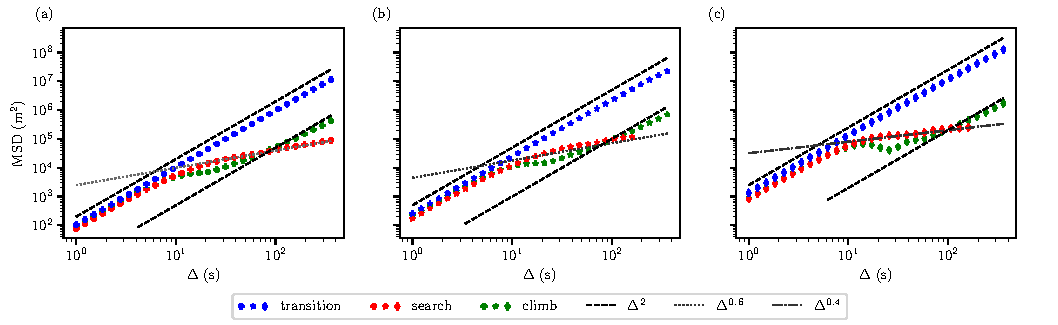
\includegraphics[width=146mm]{assets/empirical-phase-msd.pdf}};
 \head[text=glide]{8}{70}{43}{Gliding / transition}
 \head[text=search]{59}{70}{43}{Search}
 \head[text=climb]{110}{70}{43}{Climb}
 \smalltxt{8}{77}{43}{Approximately ballistic}
 \smalltxt{59}{77}{43}{Slow horizontal spreading}
 \smalltxt{110}{77}{43}{Circling with slow drift}
 \credit{Empirical reference: Vilpellet, Darmon \& Benzaquen, \href{https://arxiv.org/abs/2601.01293}{arXiv:2601.01293v1}, Fig. 3. Separate cohort from our archive.}
\finishslide
\note{These are the empirical curves in the published reference, reproduced from Figure 3. They are not new measurements on the local cleaned archive and not outputs of the earlier Pisa simulation. The three aircraft panels each contain all three phases, with blue for transition, red for search and green for climb. The figure motivates a separation between rapid horizontal relocation and slower local motion. It also shows that the horizontal displacement during search and climb is not zero.\par\medskip
Earlier work in Pisa explicitly modelled the three phases, including search and climb. The proposal now is to simplify the spatial description to gliding and an aggregate waiting state. Its adequacy has to be tested at the spatial and temporal scales of interest. Recompute the conditional MSD on the validated local labels with a documented estimator and support count. Phase survival changes the contributing population at long lags. Do not interpret a long-lag slope as asymptotic evidence without those checks.\par\medskip
Figure source: \href{https://arxiv.org/pdf/2601.01293v1}{Vilpellet et al., PDF, page 4}. The accompanying asset preserves the original vector plot and legend.}
\end{frame}

% 6 — Two-state model and a falsifiable asymptotic question.
\begin{frame}[plain]
\startslide{A two-state model with angular memory}{6 / 12}
 \smalltxt[text=teal]{8}{18}{144}{16--30 November\quad [about 2 weeks]\qquad Simplification of the earlier model developed in Pisa}
 \head[text=glide,align=center]{13}{29}{52}{Gliding}
 \smalltxt[align=center]{13}{38}{52}{$\dot{\bm r}=v(t)(\cos\theta,\sin\theta)$}
 \draw[{Stealth[length=2mm]}-{Stealth[length=2mm]},teal,line width=1pt](68,36)--(89,36);
 \head[text=ochre,align=center]{96}{29}{51}{Waiting}
 \smalltxt[align=center]{96}{38}{51}{Search + climb\\$\dot{\bm r}\simeq0$ at coarse scales}
 \ruleat{52}
 \smalltxt{8}{57}{68}{\textbf{Empirical inputs}\\Glide/wait durations, speeds and\\$C_\theta(\tau)=\langle\cos[\theta(t+\tau)-\theta(t)]\rangle$.\\Test memory within and across glides.}
 \smalltxt{84}{57}{68}{\textbf{Model test}\\Choose angular dynamics from the data.\\Can the model reproduce the full characterisation, including long-time transport?}
 \credit{Asymptotic superdiffusion is a research question. Ordinary angular Brownian motion alone has finite directional memory.}
\finishslide
\note{The earlier model in Pisa explicitly described transition, search and climb. This proposal merges search and climb into one waiting state in a coarse description of horizontal displacement. Zero waiting displacement is an approximation to test against empirical phase MSD, not an assertion that the aircraft stops. Restore drift or a local displacement term if it affects the target scales.\par\medskip
Estimate the joint distribution of durations and speeds, correlations between successive glides, and what happens to heading across a wait. Compare heading correlations in physical time and accumulated gliding time. A scalar angular Brownian motion with constant D gives exponential heading correlation for uninterrupted constant-speed flight and crosses over to ordinary diffusion. It is a baseline, not an assumed explanation of persistent asymptotic superdiffusion. Persistent angular forcing, broader duration laws or coupled states are candidate modifications only if data support them.\par\medskip
The full velocity covariance, including the state indicator and speed, controls the MSD under stationary-velocity assumptions. Appendix A2 gives the relation. Finite flight durations cannot establish an infinite-time empirical limit. Investigate the model's asymptotic law theoretically and through simulation, while validating against the measured finite range and the independent tests from stage 3.}
\end{frame}

% 7 — Candidate launches vs observed sustained association.
\begin{frame}[plain]
\startslide{Solo flight and sustained group flight}{7 / 12}
 \smalltxt[text=teal]{8}{18}{144}{30 November -- 23 December\quad [about 3 weeks + handover]}
 \head{8}{29}{40}{Candidate flights}
 \smalltxt{8}{38}{40}{Nearby launches in a common time window.\\Current viewer functionality.}
 \arrow{50}{39}{58}{39}
 \head{62}{29}{42}{Sustained association}
 \smalltxt{62}{38}{42}{Simultaneous proximity, duration and co-motion.\\Shared climb episodes.}
 \arrow{106}{39}{114}{39}
 \head[text=teal]{118}{29}{34}{Comparison}
 \smalltxt{118}{38}{34}{Reuse the stochastic tests from stage 3.}
 \ruleat{58}
 \smalltxt{8}{63}{69}{\textbf{Validation}\\Vary distance, altitude and duration thresholds. Compare with suitable surrogate pairs and manually inspect borderline cases.}
 \smalltxt{84}{63}{68}{\textbf{Controls}\\Match site/day, circuit, altitude and equipment. Treat missing nearby flights as incomplete observation of possible companions.}
 \credit{A common departure window identifies candidates. A group may form or split during flight, so labels can vary in time.}
\finishslide
\note{The current viewer uses launch cells and a time window, by default 5 km and 30 minutes. It supplies candidate cohorts, not evidence of sustained collective flight. Align absolute clocks and locations before computing horizontal and vertical separation. Define a time-resolved proximity graph and require stable proximity over a minimum duration, with checks for transitive chains. Heading or velocity alignment is informative in gliding, while shared climb episodes require a different geometry because aircraft circling the same thermal can have different instantaneous headings.\par\medskip
Thresholds should reflect measurement resolution and be checked across plausible values. Same weather and common routes can create correlated motion without social coordination. Surrogates should preserve relevant site/day and route structure while breaking actual synchrony, and should be checked for their own biases. Use ambiguous/unknown labels when coverage is poor. Recorded isolation cannot prove that a pilot had no unrecorded companions.\par\medskip
Then compare anisotropy, distributions, memory, durations and scaling, as well as pairwise correlations and separation dynamics. Report uncertainty at a dependence-aware level, such as site/day or observed group. Interpret results as associations unless a stronger causal design becomes available. Source: local \texttt{docs/guide/group-flights.md}.}
\end{frame}

% 8 — Identifiability of thermal statistics.
\begin{frame}[plain]
\startslide{What thermal statistics can the tracks reveal?}{8 / 12}
 \head[text=teal]{8}{20}{68}{An observable starting point}
 \smalltxt{8}{30}{68}{A multi-year spatial density of recorded climb locations, conditional on aircraft visits and the phase detector.}
 \smalltxt{8}{48}{68}{Estimate exposure and uncertainty. Separate repeated visits, climb events and distinct flights. Compare specific sites and terrain features.}
 \head[text=ochre]{85}{20}{67}{Quantities still to identify}
 \smalltxt{85}{30}{67}{Thermal encounter probability for a defined area and interval. Strength distribution given a location, altitude and conditions.}
 \smalltxt{85}{48}{67}{The archive alone does not identify a complete instantaneous thermal field. Similar terrain classes can hide different local structure.}
 \ruleat{64}
 \txt[font=\fontsize{12}{15}\selectfont]{8}{69}{76}{$\dot z_{\rm glider}=w_{\rm air}-s_{\rm sink}$}
 \smalltxt{85}{68}{67}{Observed climb rate is a proxy. Estimating air updraft speed needs a sink model and relevant flight conditions.}
 \credit{A normalized map of observed climbs describes sampled activity. A physical occurrence probability requires a sampling model.}
\finishslide
\note{Define the statistical object before using P(x,y). A density of sampled climb locations has units of inverse area after normalization. Climb-hours per square kilometre is an occupancy measure. A distinct-event intensity is a different object again. An occurrence probability should refer to a finite cell and time interval, at a defined altitude and under stated conditions. Pooling all years produces a historical mixture over weather, seasons and flight choices. It cannot identify a fully resolved instantaneous P(x,y,t) from these tracks alone.\par\medskip
An exposure correction can compare climbs with flight time spent sampling an area, but preferential route choice, aircraft performance and detection thresholds still affect the result. Thermal activity outside visited regions is unobserved. Two mountainous sites need not share the same distribution because slope, aspect, ridges, land cover and weather differ. Thermal tilt and advection also make height relevant to a nominally two-dimensional map.\par\medskip
For strength, w denotes vertical air velocity and s is the positive sink rate relative to the air. The approximate relation on the slide requires consistent vertical coordinates and an aircraft/polar model with bank and speed effects. Ground speed is not airspeed. The immediately observed distribution is a conditional distribution of glider climb rates. Inferring a distribution of w requires additional assumptions and uncertainty estimates. This is a research question, not a promised recovered thermal field.}
\end{frame}

% 9 — Clearly bounded exploratory control path.
\begin{frame}[plain]
\startslide{Exploratory path: stochastic optimal control}{9 / 12}
 \smalltxt[text=ochre]{8}{18}{144}{4 January -- 7 February 2027\quad [5 weeks]\qquad Scope to refine after reading and a feasibility check}
 \head{8}{29}{64}{Starting reference}
 \smalltxt{8}{38}{64}{Almgren \& Tourin study optimal speed and climb/cruise decisions under uncertain atmospheric conditions using HJB equations.}
 \smalltxt{8}{60}{64}{Possible extension: horizontal route choice in $(x,y)$, retaining altitude $z$ and the information available to the pilot.}
 \head[text=teal]{83}{29}{69}{A possible pilot study}
 \smalltxt{83}{38}{69}{1. Reproduce a simple reference problem.\\[2mm]2. Choose the state, controls and objective.\\[2mm]3. Add an empirical environmental model.\\[2mm]4. Compare policies on held-out flights.}
 \ruleat{75}
 \smalltxt{8}{78}{144}{Candidate loss: expected travel time + penalty for landing short, with a specified information set.}
 \credit{\href{https://doi.org/10.1002/oca.2122}{Almgren \& Tourin, Optimal Control Applications and Methods 36, 475--495 (2015)}. A thermal map alone is insufficient.}
\finishslide
\note{This remains the least mature path. The initial task is to study Almgren and Tourin in depth and reproduce an accessible baseline. Their paper considers optimal speed to fly and the climb/cruise free boundary, with complete foreknowledge or a Markov atmosphere revealed along the flight. It provides a starting framework rather than a ready solution for choosing routes on a two-dimensional empirical map.\par\medskip
The proposed route extension would use horizontal position plus altitude, and possibly time, environmental regime and information state. Candidate controls include heading, speed and the climb/glide decision. A finite-horizon cost could combine elapsed time with a terminal penalty for failing to reach the destination. The exact loss and constraints must follow a clear task definition and aircraft model.\par\medskip
A spatial marginal of observed climbs does not specify thermal persistence, spatial correlations, encounter rates or strength dynamics. Build those assumptions explicitly. Under uncertainty the main object is a feedback policy, with multiple possible realised trajectories, rather than a single universally optimal path. Compare travel time, completion and altitude outcomes under comparable information. An omniscient optimum is a bound, not a fair benchmark of pilot decisions. By 23 December decide whether to proceed with a limited numerical example or devote January to the model and group analysis.\par\medskip
Reference: \href{https://papers.ssrn.com/sol3/papers.cfm?abstract_id=2399214}{author-posted abstract and manuscript record}; published \href{https://doi.org/10.1002/oca.2122}{DOI 10.1002/oca.2122}.}
\end{frame}

% 10 — Dates use actual inclusive windows, plotted on a day-proportional axis.
\begin{frame}[plain]
\startslide{Indicative schedule}{10 / 12}
 \smalltxt[text=muted]{8}{18}{144}{October 2026 -- February 2027\qquad Calendar windows with approximate effort estimates.}
 \begin{scope}[xshift=60mm,yshift=-27mm,x=.65mm,y=-1mm]
  % Coordinate origin is 12 October; month boundaries are real day offsets.
  \foreach \x/\lab in {0/Oct,20/Nov,50/Dec,81/Jan,112/Feb}{
    \node[anchor=south west,inner sep=0pt,font=\fontsize{8}{10}\selectfont,text=muted]at(\x,0){\lab};
    \draw[pale](\x,2)--(\x,47);
  }
  \fill[pale!65](73,2)rectangle(84,46.5);
  \foreach \a/\b/\y/\c in {0/14/4/teal,14/35/11/teal,35/50/18/glide,49/73/25/teal,84/119/32/ochre,118/140/39/muted}{
    \fill[\c](\a,\y)rectangle(\b,\y+4);
  }
  \draw[teal,line width=1.4pt](0,48)--(140,48);
 \end{scope}
 \smalltxt{8}{30}{50}{Segmentation\quad 12/10--25/10}
 \smalltxt{8}{37}{50}{Characterisation\quad 26/10--15/11}
 \smalltxt{8}{44}{50}{Stochastic model\quad 16/11--30/11}
 \smalltxt{8}{51}{50}{Solo / group\quad 30/11--23/12}
 \smalltxt{8}{58}{50}{Optimal control\quad 04/01--07/02}
 \smalltxt{8}{65}{50}{Buffer\quad 07/02--28/02}
 \smalltxt[text=teal]{8}{72}{50}{Graphical tool\quad in parallel}
 \smalltxt[text=muted]{61}{77}{90}{24 Dec--3 Jan: break\qquad Shared handovers: 30 Nov and 7 Feb}
 \credit{Buffer: delays or deeper work on group flight, the stochastic model or optimal control, guided by the results.}
\finishslide
\note{The dates reproduce the proposed plan, with the year change made explicit. Segmentation covers 12--25 October 2026, characterisation 26 October--15 November, model work 16--30 November, and solo/group work 30 November--23 December. The model and group windows share 30 November. The group window spans 24 calendar days, so it is slightly longer than exactly three weeks. The winter break is 24 December--3 January. Optimal control covers 4 January--7 February 2027, five calendar weeks. The buffer begins on the shared 7 February milestone and continues through 28 February.\par\medskip
The bars use actual calendar-day spacing. The graphical tool runs in parallel through the whole period. The buffer is intentionally unallocated: use it for unexpected difficulties or for the most informative result, including a deeper group analysis, richer angular dynamics or a feasible control experiment. These are indicative research windows and can move after the intermediate discussions.}
\end{frame}

% 11 — Concrete, parallel tool work.
\begin{frame}[plain]
\startslide{The graphical tool as a parallel workstream}{11 / 12}
 \head[text=teal]{8}{21}{144}{One practical interface for inspection, validation and comparison}
 \head{8}{35}{40}{Easier to run}
 \smalltxt{8}{45}{40}{Documented installation, portable paths, a small example dataset and checks on another computer.}
 \head{59}{35}{42}{Easier to use}
 \smalltxt{59}{45}{42}{Clear controls and defaults, visible units, reliable loading and fewer manual setup steps.}
 \head{111}{35}{41}{Research needs}
 \smalltxt{111}{45}{41}{Review phase labels, inspect group membership and compare thermal maps and stochastic observables.}
 \ruleat{67}
 \smalltxt{8}{73}{144}{Reproducible exports should retain the cohort, filters and analysis settings used to obtain each figure.}
 \credit{Continuous maintenance and targeted additions according to the needs of stages 2--6.}
\finishslide
\note{The tool is already available and useful. The aim is to make it practical on other computers, not to promise universal compatibility without testing. Separate optional heavy data sources from the ability to run a small example. Resolve paths through configuration, document dependencies and verify the workflow on the operating systems actually used by the supervisors.\par\medskip
Add features when a research question needs them: independent label review for segmentation, synchronised group inspection, explicit definitions for thermal maps, and exports of observables with their settings and support. Usability work should reduce the number of setup steps and make loading/error states understandable. Keep the numerical analysis reproducible outside the viewer, so a screenshot can be traced to its input cohort and configuration.}
\end{frame}

% 12 — Reviewable choices, without promising every exploratory branch.
\begin{frame}[plain]
\startslide{Priorities for the supervisors' discussion}{12 / 12}
 \head[text=teal]{8}{21}{41}{Shared foundation}
 \smalltxt{8}{32}{41}{Validated segmentation and a defensible stochastic characterisation.\\[3mm]Review at the end of October and in mid-November.}
 \head[text=glide]{59}{21}{42}{Main research paths}
 \smalltxt{59}{32}{42}{An empirical test of the intermittent model.\\[3mm]A robust definition and comparison of solo/group motion.}
 \head[text=ochre]{111}{21}{41}{Conditional extension}
 \smalltxt{111}{32}{41}{Thermal inference and a limited optimal-control study.\\[3mm]Feasibility decision before the winter break.}
 \ruleat{65}
 \txt[font=\bfseries\fontsize{12}{15}\selectfont]{8}{71}{144}{February remains flexible: deepen the strongest result\\and address delays before the end of the internship.}
\finishslide
\note{The first discussion should settle the expected balance between methodological work, the stochastic model and collective flight. The core contribution is a validated framework for measuring the motion, rather than a single matched MSD exponent. The two main downstream paths can each produce a useful scientific result and can inform one another.\par\medskip
At the end of October, review segmentation accuracy and cadence coverage. In mid-November, decide which stochastic properties are supported well enough to constrain the model and group comparison. Before the winter break, decide whether thermal statistics and an accessible HJB baseline justify the January extension. If feasibility is weak, use that time to deepen stages 4 and 5. February is the explicit buffer for unfinished work or a promising result.}
\end{frame}

\appendix
% A1 — Auditable denominators and exact distinction between cadence and all gates.
\begin{frame}[plain]
\startslide{Sampling restriction: coverage and denominators}{A1}
 \smalltxt{8}{18}{144}{Archived cleaned support, segmentation export of 16 September 2026. Figures rechecked on 7 October.}
 \node[anchor=north west,inner sep=0pt,font=\fontsize{9}{11}\selectfont]at(8,29){%
 \begin{tabular}{@{}lrr@{}}
 \toprule
 & Paragliders & Hang gliders\\\midrule
 Flights in the coverage archive & \ParaTotalFlights & \HangTotalFlights\\
 Flights with any classified segment & \ParaClassFlights\ (\ParaClassFlightPct\%) & \HangClassFlights\ (\HangClassFlightPct\%)\\[1mm]
 Supported time at eligible cadence & \ParaCadTimePct\% & \HangCadTimePct\%\\
 Supported time classified, all gates & \ParaClassTimePct\% & \HangClassTimePct\%\\[1mm]
 Fixes at eligible cadence & \ParaCadFixPct\% & \HangCadFixPct\%\\
 Fixes classified, all gates & \ParaClassFixPct\% & \HangClassFixPct\%\\\bottomrule
 \end{tabular}};
 \smalltxt{8}{69}{144}{Eligible cadence: mean $\Delta t<1.2$ s. Other gates: 3,600 fixes per flight, at least 30 per segment, valid increasing timestamps.}
 \credit{Time = sum of segment end minus start, excluding gaps. Counts concern these archived cleaned segments, not all downloaded tracks.}
\finishslide
\note{The reproducible audit reads the two small phase\_coverage.parquet tables and records their SHA-256 digests in coverage-audit.json. Cadence eligibility is calculated directly from native\_cadence\_s, independently of the recorded exclusion reason. This matters because the short-flight gate fires first and can hide an additional cadence failure. The classified time uses complete spans of labelled preprocessing segments, not the sum of phase-run spans: the latter loses one interval at each phase boundary.\par\medskip
Flight percentages mean at least one qualifying segment. Fix percentages overweight densely sampled tracks compared with physical-time percentages. All three denominators must remain distinct. The displayed excluded-time percentages on slide 3 are 100 minus the all-gate classified-time percentages. These archived results do not certify accuracy, and a new preprocessing or segmentation run would require regenerating the audit.\par\medskip
The original inference extract has a reversed mapping of climb/transition in one label dictionary. The local port follows the component emissions and the original thermal-analysis scripts. This is another reason to validate behavioural labels independently, beyond numerical agreement.}
\end{frame}

% A2 — The modelling constraint used to interpret asymptotic claims.
\begin{frame}[plain]
\startslide{Angular memory and long-time transport}{A2}
 \smalltxt{8}{19}{144}{For stationary, zero-mean velocity with finite second moment:}
 \txt[font=\fontsize{14}{18}\selectfont]{17}{31}{135}{$M(\tau)=2\int_0^\tau (\tau-s)\,C_v(s)\,ds$}
 \smalltxt{17}{43}{135}{$C_v(s)=\langle\bm v(t)\cdot\bm v(t+s)\rangle$. With drift, apply this relation to centred displacement and covariance.}
 \ruleat{55}
 \smalltxt{8}{61}{68}{\textbf{Finite memory}\\If $\int_0^\infty C_v(s)\,ds$ is finite and positive, $M(\tau)\sim\tau$. Constant-speed angular Brownian motion is a baseline example.}
 \smalltxt{84}{61}{68}{\textbf{Persistent tail}\\If $C_v(s)\sim A s^{-\gamma}$, $A>0$ and $0<\gamma<1$, then $M(\tau)\sim\tau^{2-\gamma}$. Test whether the model supports this limit.}
 \credit{The velocity includes glide/wait intermittency. Heading correlation alone need not determine the full covariance.}
\finishslide
\note{The identity follows by expressing displacement as the time integral of velocity and integrating the stationary covariance over the square [0,tau] squared. For a nonzero mean velocity, the uncentred MSD also has the ballistic drift term. For nonstationary renewal dynamics, use the two-time covariance instead of this stationary reduction.\par\medskip
In uninterrupted constant-speed motion, d theta = sqrt(2D) dW yields C theta(s) = exp(-D s) and a finite correlation integral. Aggregating waiting states can change the clock and introduce duration dependence. Stationarity can fail, for example with sufficiently broad renewal waiting laws. Therefore, the empirical correlation relevant to the model is the covariance of the full velocity including state, speed and direction. The persistent-tail formula describes a sufficient asymptotic regime under the stated assumptions. It is not a claim that the finite flight archive proves that tail to infinite time.}
\end{frame}
\end{document}
